\documentclass[10pt,a4paper,oneside,BCOR5mm]{scrartcl}

%%%%%%%%%%%%%%%%%%%%%%%%%%%%%%%%%%%%%%%%%
% Arsclassica Article
% Structure Specification File
%
% This file has been downloaded from:
% http://www.LaTeXTemplates.com
%
% Original author:
% Lorenzo Pantieri (http://www.lorenzopantieri.net) with extensive modifications by:
% Vel (vel@latextemplates.com)
%
% License:
% CC BY-NC-SA 3.0 (http://creativecommons.org/licenses/by-nc-sa/3.0/)
%
%%%%%%%%%%%%%%%%%%%%%%%%%%%%%%%%%%%%%%%%%

%----------------------------------------------------------------------------------------
%	REQUIRED PACKAGES
%----------------------------------------------------------------------------------------

\usepackage[
nochapters, % Turn off chapters since this is an article        
beramono, % Use the Bera Mono font for monospaced text (\texttt)
eulermath,% Use the Euler font for mathematics
pdfspacing, % Makes use of pdftex’ letter spacing capabilities via the microtype package
dottedtoc % Dotted lines leading to the page numbers in the table of contents
]{classicthesis} % The layout is based on the Classic Thesis style

\usepackage{arsclassica} % Modifies the Classic Thesis package

\usepackage[T1]{fontenc} % Use 8-bit encoding that has 256 glyphs

\usepackage[utf8]{inputenc} % Required for including letters with accents

\usepackage{graphicx} % Required for including images
\graphicspath{{Figures/}} % Set the default folder for images

\usepackage{enumitem} % Required for manipulating the whitespace between and within lists

\usepackage{lipsum} % Used for inserting dummy 'Lorem ipsum' text into the template

\usepackage{subfig} % Required for creating figures with multiple parts (subfigures)

\usepackage{amsmath,amssymb,amsthm} % For including math equations, theorems, symbols, etc

\usepackage{varioref} % More descriptive referencing

%----------------------------------------------------------------------------------------
%	THEOREM STYLES
%---------------------------------------------------------------------------------------

\theoremstyle{definition} % Define theorem styles here based on the definition style (used for definitions and examples)
\newtheorem{definition}{Definition}

\theoremstyle{plain} % Define theorem styles here based on the plain style (used for theorems, lemmas, propositions)
\newtheorem{theorem}{Theorem}

\theoremstyle{remark} % Define theorem styles here based on the remark style (used for remarks and notes)

%----------------------------------------------------------------------------------------
%	HYPERLINKS
%---------------------------------------------------------------------------------------

\hypersetup{
%draft, % Uncomment to remove all links (useful for printing in black and white)
colorlinks=true, breaklinks=true, bookmarks=true,bookmarksnumbered,
urlcolor=webbrown, linkcolor=RoyalBlue, citecolor=webgreen, % Link colors
pdftitle={}, % PDF title
pdfauthor={\textcopyright}, % PDF Author
pdfsubject={}, % PDF Subject
pdfkeywords={}, % PDF Keywords
pdfcreator={pdfLaTeX}, % PDF Creator
pdfproducer={LaTeX with hyperref and ClassicThesis} % PDF producer
}

\pagestyle{plain}
\usepackage{makeidx}

\usepackage{fancyvrb,fancybox}
\usepackage[usenames,dvipsnames,svgnames]{xcolor}
\definecolor{gr}{RGB}{0,146,110}
\definecolor{bl}{RGB}{10,143,217}

\usepackage{type1ec}
\usepackage[english]{babel}
\usepackage{hyperref}
\hypersetup{colorlinks, citecolor=black,filecolor=black,linkcolor=black,urlcolor=black}
\usepackage{enumerate}
\usepackage{graphicx}
\usepackage{longtable}
\usepackage[T1]{fontenc}
\usepackage{ucs}
\usepackage[]{inputenc}
\usepackage{textcomp}
\usepackage{alltt}
\usepackage{listings}
\usepackage{verbatim}
\usepackage{moreverb}
\usepackage{upquote}



\usepackage{geometry}
\geometry{a4paper,left=30mm,right=30mm, top=25mm, bottom=25mm}

\lstset{language=C,basicstyle=\ttfamily,showstringspaces=false,breaklines,
numberstyle=\tiny, stepnumber=1, numbers=left,
keywordstyle=\color{blue},
commentstyle=\color{OliveGreen}, stringstyle=\color{Sepia},
rulecolor=\color{black}, xleftmargin=0.5cm, linewidth=0.95\textwidth}

 \setlength{\parskip}{1ex plus 0.5ex minus 0.2ex}

\makeatletter
\DeclareRobustCommand*\textsubscript[1]{%
  \@textsubscript{\selectfont#1}}
\def\@textsubscript#1{%
  {\m@th\ensuremath{_{\mbox{\fontsize\sf@size\z@#1}}}}}
\makeatother

\title{AsciiDoc \&{} Latex}
\author{Martin Horauer}
\date{2014}
\publishers{\begin{tabular}{ll}    \end{tabular}}


\newenvironment{packed_enum}{
\begin{itemize}
  \setlength{\itemsep}{-5pt}
  \setlength{\parskip}{0pt}
  \setlength{\parsep}{0pt}
}{\end{itemize}}


\author{\spacedlowsmallcaps{Martin Horauer}}
\date{2014}

\usepackage{scrpage2}
\pagestyle{scrheadings}
\usepackage[xindy]{imakeidx}
\indexsetup{noclearpage,columns=2,firstpagestyle=scrheadings}
\makeindex

\begin{document}
\renewcommand{\sectionmark}[1]{\markright{\spacedlowsmallcaps{#1}}}
\lehead{\mbox{\llap{\small\thepage\kern1em\color{halfgray} \vline}\color{halfgray}\hspace{0.5em}\rightmark\hfil}}
\label{header}\hypertarget{header}{}
\maketitle
\setcounter{tocdepth}{2}
\tableofcontents
\section*{About}
\textcopyright{} by Martin Horauer; some rights reserved. 
A PDF of this document can be downloaded for free from 
\url{http://embsys.technikum-wien.at/staff/horauer}.


\hypertarget{_preface}{}
\section{Preface}
\label{_preface}
 \par\noindent{}Prerequisites for this chapter are
  \begin{itemize}
\item%
familiarity with the C programming language and how to build programs on the command-line

\item%
electronic fundamentals like know how to dimension small circuits

\item%
\dots{}

\end{itemize}
 \par\noindent{}When working through this chapter you shall be able to
  \begin{itemize}
\item%
efficiently read and understand data-sheets and user-manuals of micro-controllers

\item%
know about registers and how to access them

\item%
\dots{}

\end{itemize}
\hypertarget{_page_layout}{}
\chapter{Page Layout}
\label{_page_layout}
 \par\noindent{}Arsclassica-\LaTeX{} is an article style, thus using AsciiDoc one will need to stick to the top-level heading styles set with \texttt{==}, \texttt{===}, etc. respectively.
 \par\noindent{}\index{heading}
\index{heading!levels}
\index{heading!levels!section}
\index{heading!levels!subsection}
\hypertarget{_images_and_figures}{}
\section{Images and Figures}
\label{_images_and_figures}
 \par\noindent{}\index{figures}
Expect the \emph{usual} quirks with figures in \LaTeX{} and all word processing tools. You'll eventually need to move the figures around in order to get an optimal placement.
\begin{figure}[!htbp]
\begin{center}
\hypertarget{figsine}{}
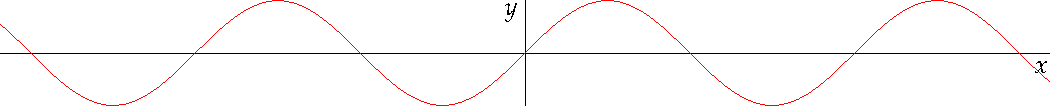
\includegraphics[scale=.8,]{source/sine.pdf}%
\label{figsine}
\caption{This graph shows y = sin x from about x = [-10, 10]. \emph{Notice that this figure takes up the full page width.}}
\end{center}
\end{figure}
 \par\noindent{}Figure \hyperlink{figsine}{1} spans the entire page width by default. The figures caption is derived from the image block title. The figure itself set using \texttt{image::sine.\{{}imgext\}{}[]}.
 \par\noindent{}In order to scale figures you may use the \texttt{scale}  or the \texttt{width} parameter, e.g.:
\begin{alltt}.Hilbercurves 115\%{} scaled
image::source/hilbertcurves.\{{}imgext\}{}[scale=\textquotedbl{}.115\textquotedbl{}]\end{alltt}
 \par\noindent{}\index{figures!scaling}
\begin{figure}[!htbp]
\begin{center}
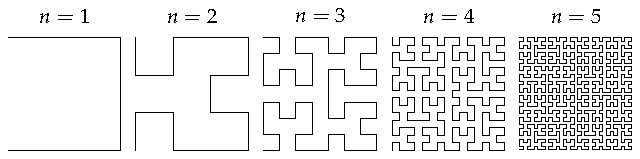
\includegraphics[scale=1.15,]{source/hilbertcurves.pdf}%
\caption{Hilbercurves 115\%{} scaled}
\end{center}
\end{figure}
\hypertarget{_code_listings}{}
\section{Code Listings}
\label{_code_listings}
 \par\noindent{}Code snippets are set using the \texttt{lstlisting} package. The following example illustrates the respective output of the following AsciiDoc snippet:
\begin{alltt}.Hello World Example
[source,c,numbered]
----
include::source/hello.c[]
----\end{alltt}
 \par\noindent{}In this case the parameter \texttt{c} is passed on to the \texttt{lstlisting} package to select the appropriate language.
\begin{figure*}[!hptb]
\begin{lstlisting}[caption=Hello World Example,language=c,frame=L]
// the usual 'hello world' example in C
#include <stdio.h>

int main(void)
{
    printf("Hello World!\n");
    return 0;
}\end{lstlisting}
\end{figure*}
\hypertarget{_verbatim_input}{}
\section{Verbatim Input}
\label{_verbatim_input}
 \par\noindent{}To describe commands entered at a terminal prompt we adapt a \texttt{verbatim} environment. Respective code is set between multiple dots and results in an output as in the following example.
\begin{alltt}\%{} ls
tufte.txt latex.conf\end{alltt}
\hypertarget{_tables}{}
\section{Tables}
\label{_tables}
 \par\noindent{}The following AsciiDoc snippet generates table \hyperlink{tab1}{1}.
\begin{alltt}.Table Example
[format=\textquotedbl{}csv\textquotedbl{},options=\textquotedbl{}header\textquotedbl{},frame=\textquotedbl{}all\textquotedbl{},colspecs=\textquotedbl{}clllr\textquotedbl{}]
\textbar{}===================================================
ID,Customer Name,Contact Name,Phone
include::source/data.csv[]
\textbar{}===================================================\end{alltt}
 \par\noindent{}Here the parameter \texttt{colspecs} specifies the alignment of the columns (c \dots{} center, l \dots{} left, r \dots{} right). Vertical lines can be drawn using a \texttt{\textbar{}} between colspecs arguments; with the used \texttt{booktabs} package, however, this usually renders an inferior looking output. The argument \texttt{frame} supports either \texttt{all} or \texttt{topbot} as values. The first one renders three horizontal lines as illustrated in Tab. \hyperlink{tab1}{1}, whereas the latter only renders a horizontal line above and below the table.
Finally, using the value \texttt{header} for the argument \texttt{options} draws the first line in bold letters.
  \begin{table}[!hptb]
  \begin{center}
 \hypertarget{tab1}{}
 \caption{Table Example}
 \begin{tabular}{
 clllr
 }
 \hline
 
{\bfseries{}ID} &
{\bfseries{}Customer Name} &
{\bfseries{}Contact Name} &
{\bfseries{}Phone} 
 \tabularnewline
 
AROUT &
Around the Horn &
Thomas Hardy &
(171) 555-7788 %
 \tabularnewline

BERGS &
Berglunds snabbkop &
Christina Berglund &
0921-12 34 65 %
 \tabularnewline

BLAUS &
Blauer See Delikatessen &
Hanna Moos &
0621-08460 %
 \tabularnewline
 \hline
 \end{tabular}
  \end{center}
 \label{tab1}
  \end{table}
\hypertarget{_miscellaneous}{}
\chapter{Miscellaneous}
\label{_miscellaneous}
 \par\noindent{}This section presents several items like admonitions, quotes, etc.
\hypertarget{_admonitions}{}
\section{Admonitions}
\label{_admonitions}
 \par\noindent{}Admonitions are small paragraphs that try to highlight something. Often admonitions are set along with a small icon and try to state either a \texttt{NOTE},
\texttt{TIP}, \texttt{IMPORTANT}, \texttt{WARNING}, or \texttt{CAUTION} statement. \newline{}
\begin{addmargin*}[0em]{0em}
\vspace*{2mm}
\fcolorbox{bl}{white}{
\begin{minipage}{.07\linewidth}

\includegraphics[width=7mm]{./images/icons/note.pdf}
\end{minipage}
%
\begin{minipage}{.9\linewidth}
%\color{OliveGreen}
\parbox{0.9\linewidth}{Place the admonition just below the text where you want the block to show up.}
%\color{black}
\end{minipage}
}
\vspace*{2mm}
\end{addmargin*}
 \par\noindent{}The following AsciiDoc code produces the admonition shown in the margin.
\begin{alltt}[\textquotedbl{}NOTE\textquotedbl{}]
Place the admonition just below the text where you
want the block to show up.\end{alltt}
 \par\noindent{}For \texttt{TIP}, \texttt{IMPORTANT}, \texttt{WARNING}, or \texttt{CAUTION} you'll get different icons. All icons reside in the \texttt{images/icons/} folder are included as \emph{.pdf} images into the \LaTeX{} output.
\hypertarget{_quotes}{}
\section{Quotes}
\label{_quotes}
 \par\noindent{}In the following we show a simple quotation from Johann Wolfgang von Goethe.
\begin{quote}

 \par\noindent{}There is nothing more dreadful than imagination without taste.

\end{quote}

\begin{flushright}
-- Johann Wolfgang von Goethe
\end{flushright}
 \par\noindent{}It is set in AsciiDoc using underscores:
\begin{alltt}[quote, Johann Wolfgang von Goethe]
\_{}\_{}\_{}\_{}
There is nothing more dreadful than imagination without taste.
\_{}\_{}\_{}\_{}\end{alltt}
\hypertarget{_links}{}
\section{Links}
\label{_links}
 \par\noindent{}Frequently usedf links are, e.g., URLs like \href{http://www.horauer.at/}{horauer.at} or mailto references (e.g. \href{mailto:mhorauer@gmail.com}{email Martin Horauer}). In AsciiDoc simply write:
\begin{alltt}http://www.horauer.at/[horauer.at]
mailto:mhorauer@gmail.com[email Martin Horauer]\end{alltt}
 \par\noindent{}For the use of local references one uses \label{anchors}\hypertarget{anchors}{anchors} (set using \texttt{[[anchors]]}) and references (set using \texttt{\textless{}\textless{}anchor,ref\textgreater{}\textgreater{}}) where \texttt{ref} is the actual displayed \hyperlink{anchor}{ref} of the respective hyperlink.
\hypertarget{_bibliographies}{}
\section{Bibliographies}
\label{_bibliographies}
 \par\noindent{}In order to add a bibliography add a block like the following one after the body of the text:
\begin{alltt}[bibliography]
- [[[tufte01]]] Edward R. Tufte.
'The Visual Display of Quantitative Information'.
Graphics Press, Cheshire, Connecticut, 2001.
ISBN 0-9613921-4-2.\end{alltt}
\begin{addmargin*}[0em]{0em}
\vspace*{2mm}
\fcolorbox{bl}{white}{
\begin{minipage}{.07\linewidth}

\includegraphics[width=7mm]{./images/icons/caution.pdf}
\end{minipage}
%
\begin{minipage}{.9\linewidth}
%\color{OliveGreen}
\parbox{0.9\linewidth}{The \texttt{natbib} style used generates a warning message that can be safely ignored.}
%\color{black}
\end{minipage}
}
\vspace*{2mm}
\end{addmargin*}
\hypertarget{_indices}{}
\section{Indices}
\label{_indices}
 \par\noindent{}In order to generate an index enclose selected words within the text in double parentheses. When you want to place index entries at pages, that are hidden in the text, use triple parenthesis.
Furthermore, in order to subclass index entries use commas, e.g.:
\begin{alltt}((heading))            \#{} index entry where heading is visible in the text
(((heading)))          \#{} index entry where heading is invisible
(((heading,levels)))   \#{} invisible index entry with a sub-element\end{alltt}
 \par\noindent{}In order to insert the index create an empty index section at the end of the document, e.g.:
\begin{alltt}[index]
== Index

////////////////////////////////////////////////////////////////
The index is normally left completely empty, it's contents being
generated automatically by the makeindex command.
////////////////////////////////////////////////////////////////\end{alltt}
 \par\noindent{}Finally, to generate the index entries run:
\begin{alltt}\%{} pdflatex tufte
\%{} makeindex tufte
\%{} pdflatex tufte\end{alltt}
\label{_references}\hypertarget{_references}{}
\begin{thebibliography}{99}
  \begin{bibliography} 

\bibitem{tufte01}  \label{tufte01}\hypertarget{tufte01}{} Edward R. Tufte.
\emph{The Visual Display of Quantitative Information}.
Graphics Press, Cheshire, Connecticut, 2001.
ISBN 0-9613921-4-2. \newline{}


\bibitem{tufte06}  \label{tufte06}\hypertarget{tufte06}{} Edward R. Tufte. \emph{Beautiful Evidence}.
Graphics Press, Cheshire, Connecticut, 2006.
ISBN 0-9613921-7-7.

 \end{bibliography}
\end{thebibliography}
\setindexpreamble{
}
\label{_index}\hypertarget{_index}{}
\printindex
\label{footer}\hypertarget{footer}{}
\end{document}
